\documentclass{controle}
\usepackage{main}

\title{Évaluation n°9: Inéquations de la forme $f(x) < g(x)$}
\date{15 Décembre 2025}
\author{Seconde 3}

\begin{document}
\maketitle
\version
\begin{questions}
\titledquestion{} Soient $f$ et $g$ deux fonctions définies sur $[-8;8]$ dont les courbes représentatives sont données sur le repère suivant :
\begin{center}
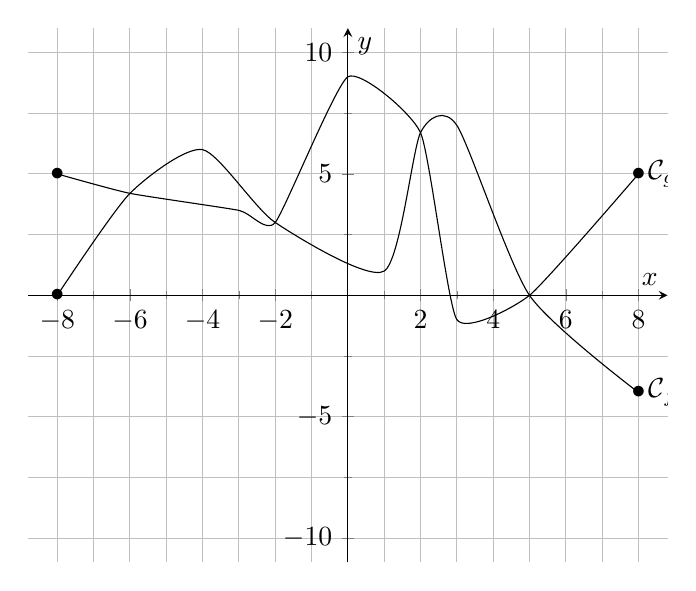
\begin{tikzpicture}
\begin{axis}[
  grid=both,
  axis lines=middle,
  enlarge x limits=0.05,
  enlarge y limits=0.05,
  xmin=-8,
  xmax=8,
  ymin=-10,
  ymax=10,
  xlabel={$x$},
  ylabel={$y$},
  width=0.8\textwidth,
  minor tick num=1]
\addplot[smooth,tension=0.4] coordinates {(-8,0) (-6,4.2) (-4,6) (-2,3) (1,1) (2,6.7) (3,7) (5,0) (8,-4)} 
  node[pos=1, right] {$\mathcal{C}_f$} 
  node[pos=1] {$\bullet$}
  node[pos=0] {$\bullet$};
\addplot[smooth,tension=0.3] coordinates {(-8,5) (-6,4.2) (-3,3.5) (-2,3) (0,9) (2,6.7) (3,-1) (5,0) (8,5)} 
  node[pos=1, right] {$\mathcal{C}_g$} 
  node[pos=1] {$\bullet$}
  node[pos=0] {$\bullet$};
\end{axis}
\end{tikzpicture}
\end{center}
\begin{parts}
\part Résoudre graphiquement l'équation $f(x) = g(x)$. \textbf{On précisera l'ensemble $S$ des solutions.}
\part Résoudre graphiquement l'inéquation $f(x) \leq g(x)$. \textbf{On précisera l'ensemble $S$ des solutions.}
\part Résoudre graphiquement l'inéquation $f(x) > g(x)$. \textbf{On précisera l'ensemble $S$ des solutions.}
\end{parts}
\end{questions}
\newpage
\maketitle
\version
\begin{questions}
\titledquestion{} Soient $f$ et $g$ deux fonctions définies sur $[-8;8]$ dont les courbes représentatives sont données sur le repère suivant :
\begin{center}
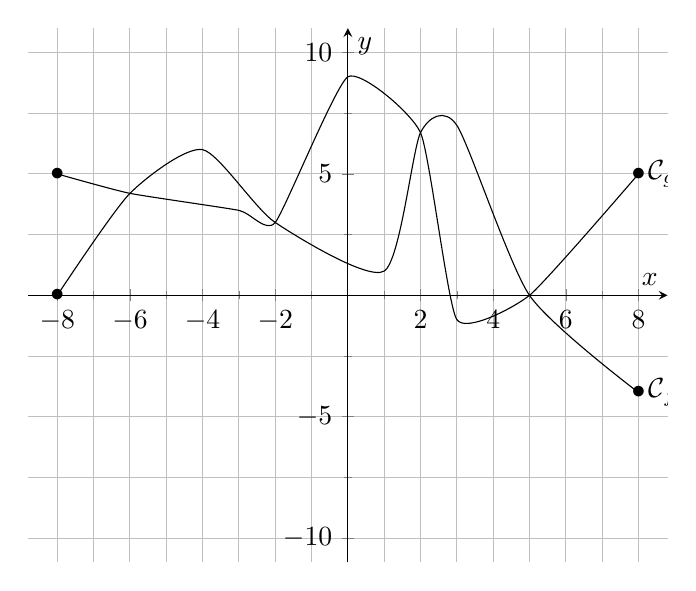
\begin{tikzpicture}
\begin{axis}[
  grid=both,
  axis lines=middle,
  enlarge x limits=0.05,
  enlarge y limits=0.05,
  xmin=-8,
  xmax=8,
  ymin=-10,
  ymax=10,
  xlabel={$x$},
  ylabel={$y$},
  width=0.8\textwidth,
  minor tick num=1]
\addplot[smooth,tension=0.4] coordinates {(-8,0) (-6,4.2) (-4,6) (-2,3) (1,1) (2,6.7) (3,7) (5,0) (8,-4)} 
  node[pos=1, right] {$\mathcal{C}_f$} 
  node[pos=1] {$\bullet$}
  node[pos=0] {$\bullet$};
\addplot[smooth,tension=0.3] coordinates {(-8,5) (-6,4.2) (-3,3.5) (-2,3) (0,9) (2,6.7) (3,-1) (5,0) (8,5)} 
  node[pos=1, right] {$\mathcal{C}_g$} 
  node[pos=1] {$\bullet$}
  node[pos=0] {$\bullet$};
\end{axis}
\end{tikzpicture}
\end{center}
\begin{parts}
\part Résoudre graphiquement l'équation $f(x) = g(x)$. \textbf{On précisera l'ensemble $S$ des solutions.}
\part Résoudre graphiquement l'inéquation $f(x) \leq g(x)$. \textbf{On précisera l'ensemble $S$ des solutions.}
\part Résoudre graphiquement l'inéquation $f(x) > g(x)$. \textbf{On précisera l'ensemble $S$ des solutions.}
\end{parts}
\end{questions}
\end{document}